% coding:utf-8

%FOSAET, a LaTeX-Code for a electrical summary of basic electronics
%Copyright (C) 2013, Daniel Winz, Ervin Mazlagic, Mario Felder

%This program is free software; you can redistribute it and/or
%modify it under the terms of the GNU General Public License
%as published by the Free Software Foundation; either version 2
%of the License, or (at your option) any later version.

%This program is distributed in the hope that it will be useful,
%but WITHOUT ANY WARRANTY; without even the implied warranty of
%MERCHANTABILITY or FITNESS FOR A PARTICULAR PURPOSE.  See the
%GNU General Public License for more details.
%----------------------------------------

\subsection{Source Schaltung mit Spannungsgegenkopplung}
\begin{figure}[h!]
	\centering
	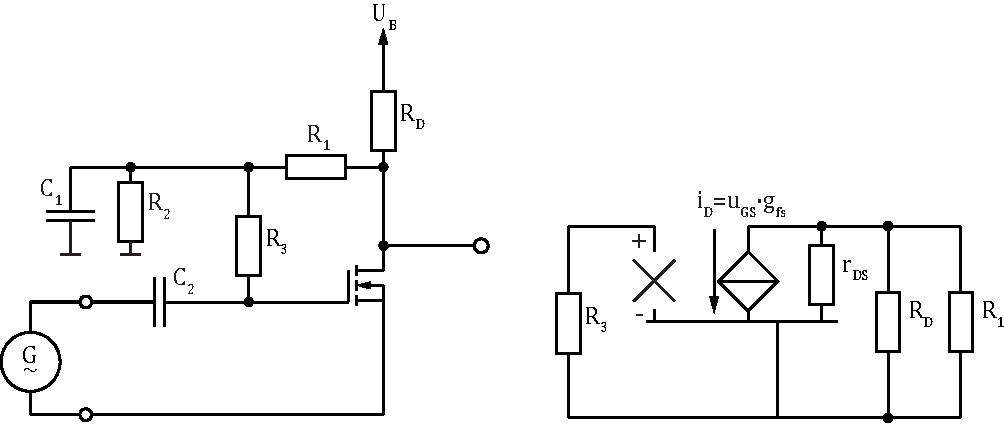
\includegraphics[width = \linewidth]{../fig/fet_source_u.pdf}
	\caption{Source Schaltung mit Spannungsgegenkopplung und Kleinsignalersatzschaltung}
	\label{fet:sourceschaltung_u}
\end{figure}
\noindent
\paragraph{Dimensionierung:}
\begin{itemize}
	\item Wahl von $I_D$ aufgrund des nötigen Ausgangswiderstandes $\rightarrow R_D$
	\item Wahl von $R_3$ im Bereich von $100k\Omega$ bis $10M\Omega$
	\item $R_1 \approx 100\cdot R_D$
	\item $R_2 = R_1 \cdot \frac{U_{GS}}{(U_a-U_{GS})}$
	\item Untere Grenfrequenz: $f_{gu} = \frac{1}{2\pi \cdot R_3 \cdot C_2}$
	\item Wahl von $C_1$ dass $C_1 \cdot R_1 \parallel R_2 \gg C_2 \cdot R_3$
\end{itemize}
